\documentclass[]{article}
\usepackage{lmodern}
\usepackage{amssymb,amsmath}
\usepackage{ifxetex,ifluatex}
\usepackage{fixltx2e} % provides \textsubscript
\ifnum 0\ifxetex 1\fi\ifluatex 1\fi=0 % if pdftex
  \usepackage[T1]{fontenc}
  \usepackage[utf8]{inputenc}
\else % if luatex or xelatex
  \ifxetex
    \usepackage{mathspec}
  \else
    \usepackage{fontspec}
  \fi
  \defaultfontfeatures{Ligatures=TeX,Scale=MatchLowercase}
\fi
% use upquote if available, for straight quotes in verbatim environments
\IfFileExists{upquote.sty}{\usepackage{upquote}}{}
% use microtype if available
\IfFileExists{microtype.sty}{%
\usepackage{microtype}
\UseMicrotypeSet[protrusion]{basicmath} % disable protrusion for tt fonts
}{}
\usepackage[margin=1in]{geometry}
\usepackage{hyperref}
\hypersetup{unicode=true,
            pdfborder={0 0 0},
            breaklinks=true}
\urlstyle{same}  % don't use monospace font for urls
\usepackage{color}
\usepackage{fancyvrb}
\newcommand{\VerbBar}{|}
\newcommand{\VERB}{\Verb[commandchars=\\\{\}]}
\DefineVerbatimEnvironment{Highlighting}{Verbatim}{commandchars=\\\{\}}
% Add ',fontsize=\small' for more characters per line
\usepackage{framed}
\definecolor{shadecolor}{RGB}{248,248,248}
\newenvironment{Shaded}{\begin{snugshade}}{\end{snugshade}}
\newcommand{\AlertTok}[1]{\textcolor[rgb]{0.94,0.16,0.16}{#1}}
\newcommand{\AnnotationTok}[1]{\textcolor[rgb]{0.56,0.35,0.01}{\textbf{\textit{#1}}}}
\newcommand{\AttributeTok}[1]{\textcolor[rgb]{0.77,0.63,0.00}{#1}}
\newcommand{\BaseNTok}[1]{\textcolor[rgb]{0.00,0.00,0.81}{#1}}
\newcommand{\BuiltInTok}[1]{#1}
\newcommand{\CharTok}[1]{\textcolor[rgb]{0.31,0.60,0.02}{#1}}
\newcommand{\CommentTok}[1]{\textcolor[rgb]{0.56,0.35,0.01}{\textit{#1}}}
\newcommand{\CommentVarTok}[1]{\textcolor[rgb]{0.56,0.35,0.01}{\textbf{\textit{#1}}}}
\newcommand{\ConstantTok}[1]{\textcolor[rgb]{0.00,0.00,0.00}{#1}}
\newcommand{\ControlFlowTok}[1]{\textcolor[rgb]{0.13,0.29,0.53}{\textbf{#1}}}
\newcommand{\DataTypeTok}[1]{\textcolor[rgb]{0.13,0.29,0.53}{#1}}
\newcommand{\DecValTok}[1]{\textcolor[rgb]{0.00,0.00,0.81}{#1}}
\newcommand{\DocumentationTok}[1]{\textcolor[rgb]{0.56,0.35,0.01}{\textbf{\textit{#1}}}}
\newcommand{\ErrorTok}[1]{\textcolor[rgb]{0.64,0.00,0.00}{\textbf{#1}}}
\newcommand{\ExtensionTok}[1]{#1}
\newcommand{\FloatTok}[1]{\textcolor[rgb]{0.00,0.00,0.81}{#1}}
\newcommand{\FunctionTok}[1]{\textcolor[rgb]{0.00,0.00,0.00}{#1}}
\newcommand{\ImportTok}[1]{#1}
\newcommand{\InformationTok}[1]{\textcolor[rgb]{0.56,0.35,0.01}{\textbf{\textit{#1}}}}
\newcommand{\KeywordTok}[1]{\textcolor[rgb]{0.13,0.29,0.53}{\textbf{#1}}}
\newcommand{\NormalTok}[1]{#1}
\newcommand{\OperatorTok}[1]{\textcolor[rgb]{0.81,0.36,0.00}{\textbf{#1}}}
\newcommand{\OtherTok}[1]{\textcolor[rgb]{0.56,0.35,0.01}{#1}}
\newcommand{\PreprocessorTok}[1]{\textcolor[rgb]{0.56,0.35,0.01}{\textit{#1}}}
\newcommand{\RegionMarkerTok}[1]{#1}
\newcommand{\SpecialCharTok}[1]{\textcolor[rgb]{0.00,0.00,0.00}{#1}}
\newcommand{\SpecialStringTok}[1]{\textcolor[rgb]{0.31,0.60,0.02}{#1}}
\newcommand{\StringTok}[1]{\textcolor[rgb]{0.31,0.60,0.02}{#1}}
\newcommand{\VariableTok}[1]{\textcolor[rgb]{0.00,0.00,0.00}{#1}}
\newcommand{\VerbatimStringTok}[1]{\textcolor[rgb]{0.31,0.60,0.02}{#1}}
\newcommand{\WarningTok}[1]{\textcolor[rgb]{0.56,0.35,0.01}{\textbf{\textit{#1}}}}
\usepackage{graphicx,grffile}
\makeatletter
\def\maxwidth{\ifdim\Gin@nat@width>\linewidth\linewidth\else\Gin@nat@width\fi}
\def\maxheight{\ifdim\Gin@nat@height>\textheight\textheight\else\Gin@nat@height\fi}
\makeatother
% Scale images if necessary, so that they will not overflow the page
% margins by default, and it is still possible to overwrite the defaults
% using explicit options in \includegraphics[width, height, ...]{}
\setkeys{Gin}{width=\maxwidth,height=\maxheight,keepaspectratio}
\IfFileExists{parskip.sty}{%
\usepackage{parskip}
}{% else
\setlength{\parindent}{0pt}
\setlength{\parskip}{6pt plus 2pt minus 1pt}
}
\setlength{\emergencystretch}{3em}  % prevent overfull lines
\providecommand{\tightlist}{%
  \setlength{\itemsep}{0pt}\setlength{\parskip}{0pt}}
\setcounter{secnumdepth}{0}
% Redefines (sub)paragraphs to behave more like sections
\ifx\paragraph\undefined\else
\let\oldparagraph\paragraph
\renewcommand{\paragraph}[1]{\oldparagraph{#1}\mbox{}}
\fi
\ifx\subparagraph\undefined\else
\let\oldsubparagraph\subparagraph
\renewcommand{\subparagraph}[1]{\oldsubparagraph{#1}\mbox{}}
\fi

%%% Use protect on footnotes to avoid problems with footnotes in titles
\let\rmarkdownfootnote\footnote%
\def\footnote{\protect\rmarkdownfootnote}

%%% Change title format to be more compact
\usepackage{titling}

% Create subtitle command for use in maketitle
\providecommand{\subtitle}[1]{
  \posttitle{
    \begin{center}\large#1\end{center}
    }
}

\setlength{\droptitle}{-2em}

  \title{}
    \pretitle{\vspace{\droptitle}}
  \posttitle{}
    \author{}
    \preauthor{}\postauthor{}
    \date{}
    \predate{}\postdate{}
  

\begin{document}

\hypertarget{calculo-de-las-matrices-de-transicion}{%
\subsection{5 Cálculo de las matrices de
transición}\label{calculo-de-las-matrices-de-transicion}}

Se realizaron los cálculos de la matriz de transición para los puesto
metereológicos de Milpo, Pira y Recuay. Todos ellos dentro del
departamento de Ancash. El proceso se realizó haciendo uso de R y se
detalla a continuación:

Los dataset fueron extraídos de la página web del Senahmi.

\begin{Shaded}
\begin{Highlighting}[]
\CommentTok{#Cargar los datasets}
\NormalTok{milpo<-}\KeywordTok{read.table}\NormalTok{(}\StringTok{"milpo.txt"}\NormalTok{, }\DataTypeTok{header =} \OtherTok{FALSE}\NormalTok{, }\DataTypeTok{sep =} \StringTok{" "}\NormalTok{, }\DataTypeTok{dec =}\StringTok{"."}\NormalTok{)}
\NormalTok{pira<-}\KeywordTok{read.table}\NormalTok{(}\StringTok{"pira.txt"}\NormalTok{, }\DataTypeTok{header =} \OtherTok{FALSE}\NormalTok{, }\DataTypeTok{sep =} \StringTok{" "}\NormalTok{, }\DataTypeTok{dec =}\StringTok{"."}\NormalTok{)}
\NormalTok{recuay<-}\KeywordTok{read.table}\NormalTok{(}\StringTok{"recuay.txt"}\NormalTok{, }\DataTypeTok{header =} \OtherTok{FALSE}\NormalTok{, }\DataTypeTok{sep =} \StringTok{" "}\NormalTok{, }\DataTypeTok{dec =} \StringTok{"."}\NormalTok{)}
\end{Highlighting}
\end{Shaded}

\begin{Shaded}
\begin{Highlighting}[]
\CommentTok{#Cambiar los datos faltantes por NA}
\NormalTok{milpo[milpo}\OperatorTok{==-}\FloatTok{99.9}\NormalTok{]<-}\OtherTok{NA}
\NormalTok{pira[pira}\OperatorTok{==-}\FloatTok{99.9}\NormalTok{]<-}\OtherTok{NA}
\NormalTok{recuay[recuay}\OperatorTok{==-}\FloatTok{99.9}\NormalTok{]<-}\OtherTok{NA}
\end{Highlighting}
\end{Shaded}

A continuación se muestran gráficos que resumen la data que se está
utilizando:

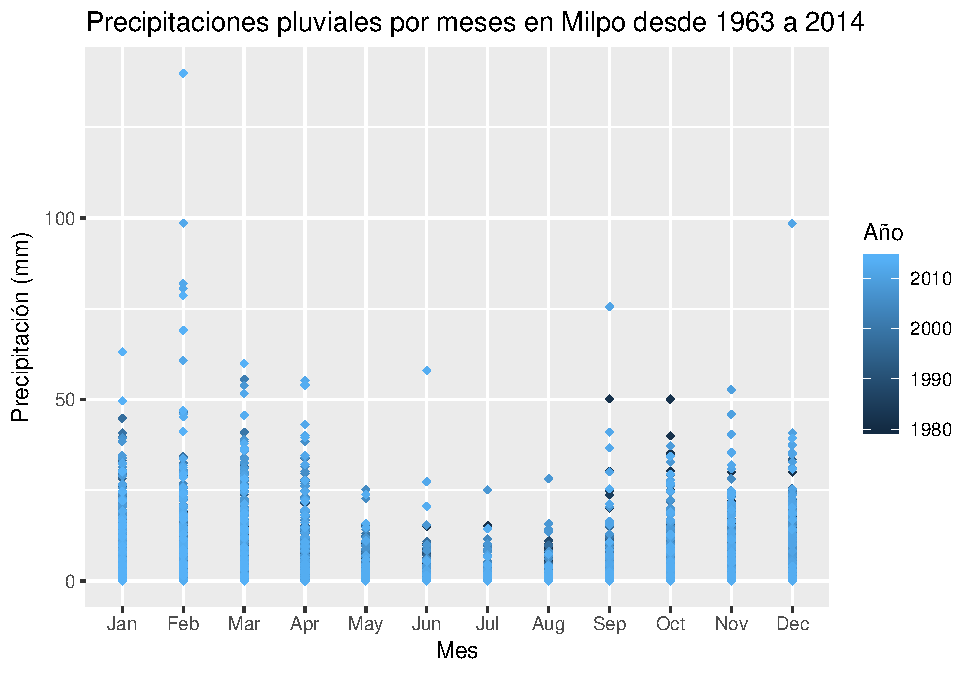
\includegraphics{proyecto_files/figure-latex/unnamed-chunk-5-1.pdf}
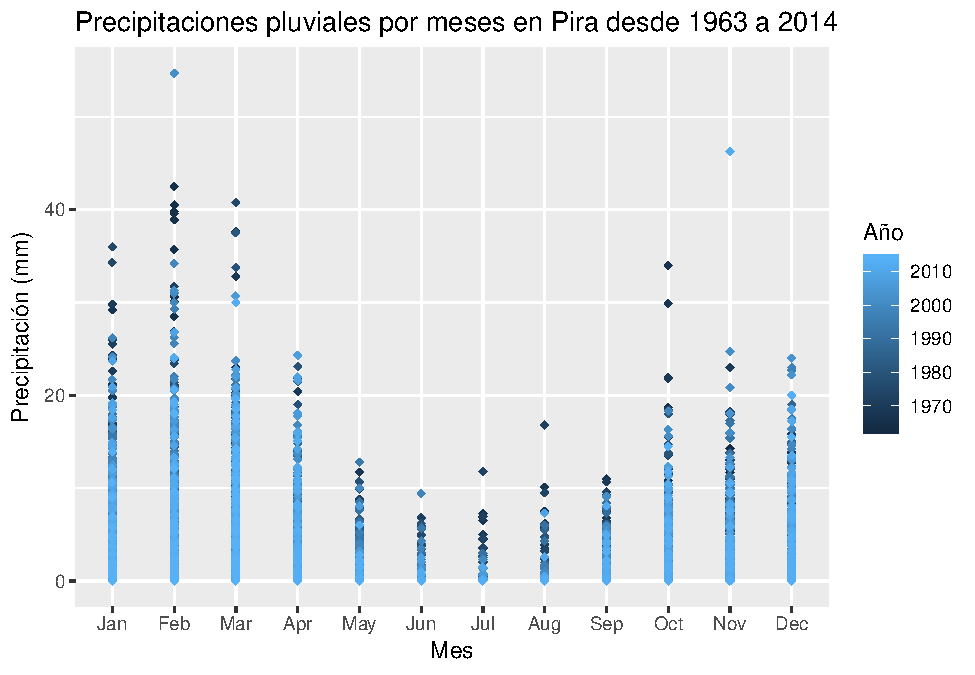
\includegraphics{proyecto_files/figure-latex/unnamed-chunk-5-2.pdf}
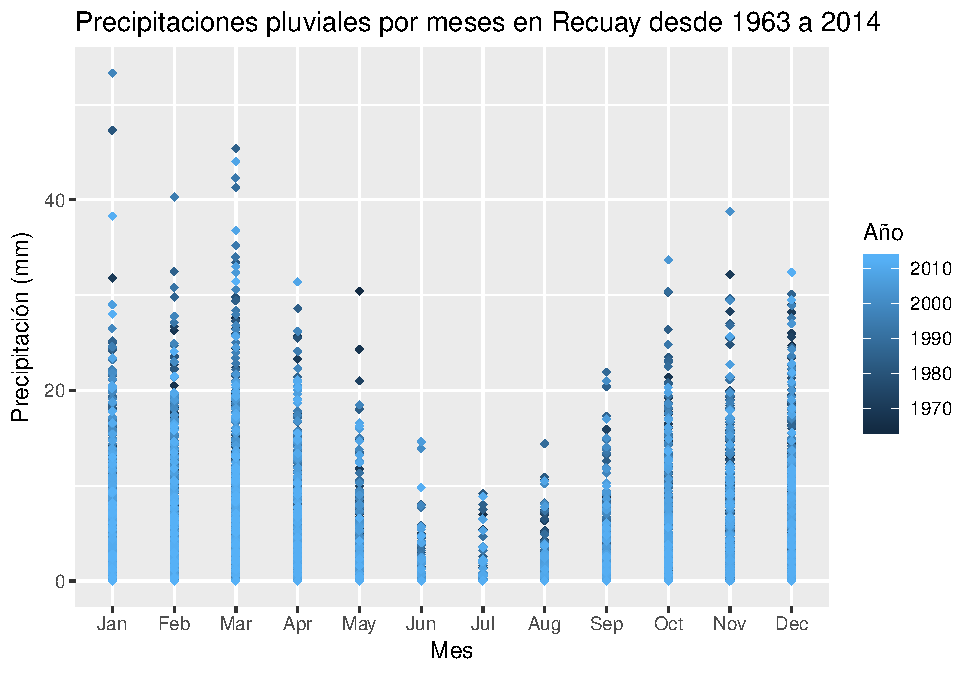
\includegraphics{proyecto_files/figure-latex/unnamed-chunk-5-3.pdf}

También se genera un gráfico de un año promedio para cada una de las
estaciones metereológicas consideradas en el estudio:

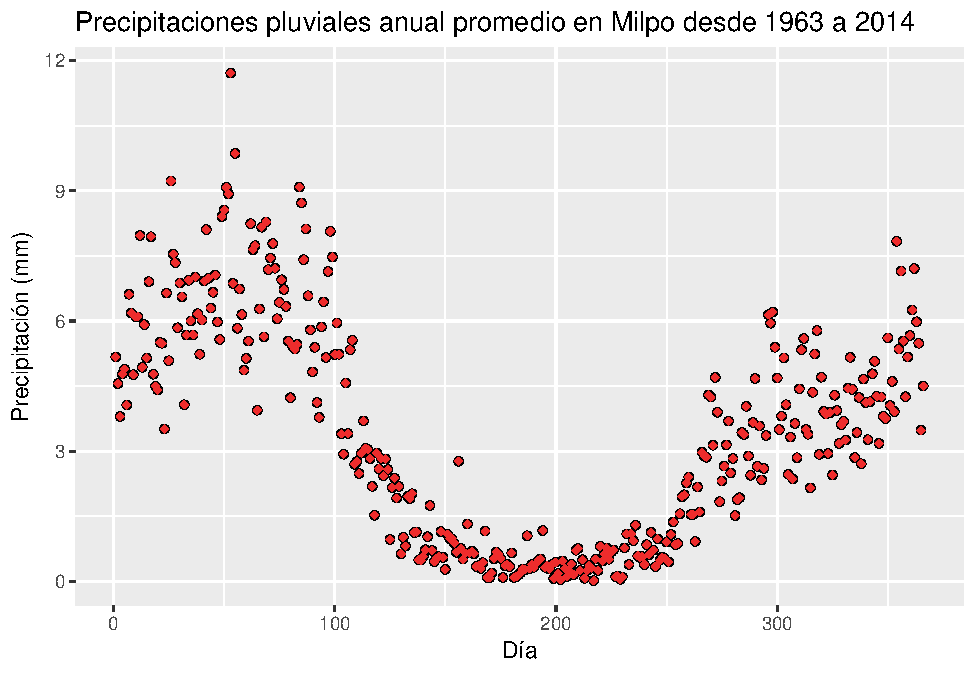
\includegraphics{proyecto_files/figure-latex/unnamed-chunk-6-1.pdf}
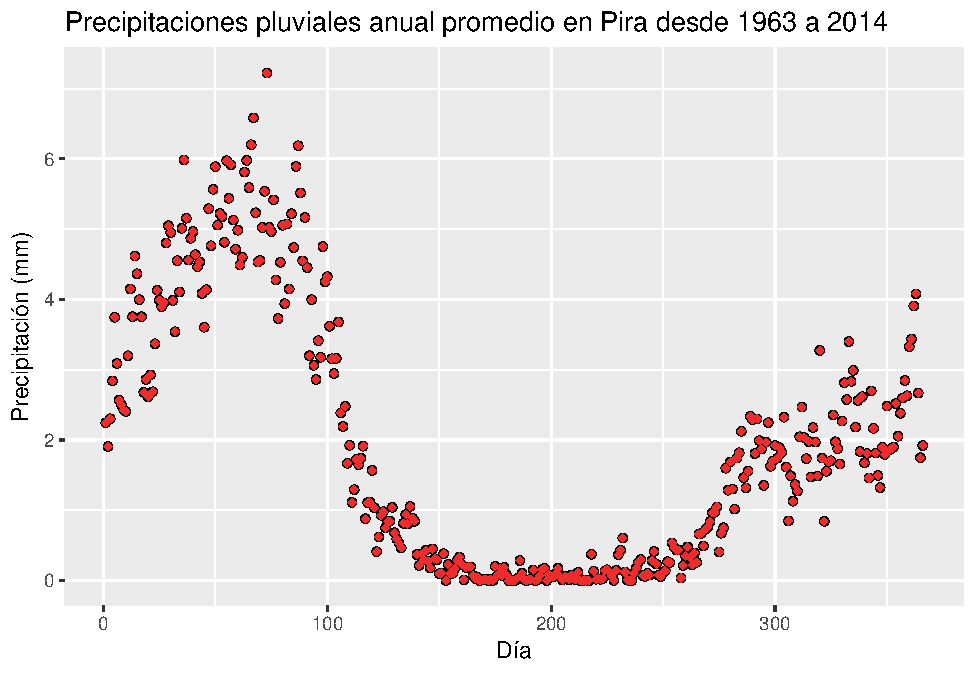
\includegraphics{proyecto_files/figure-latex/unnamed-chunk-6-2.pdf}
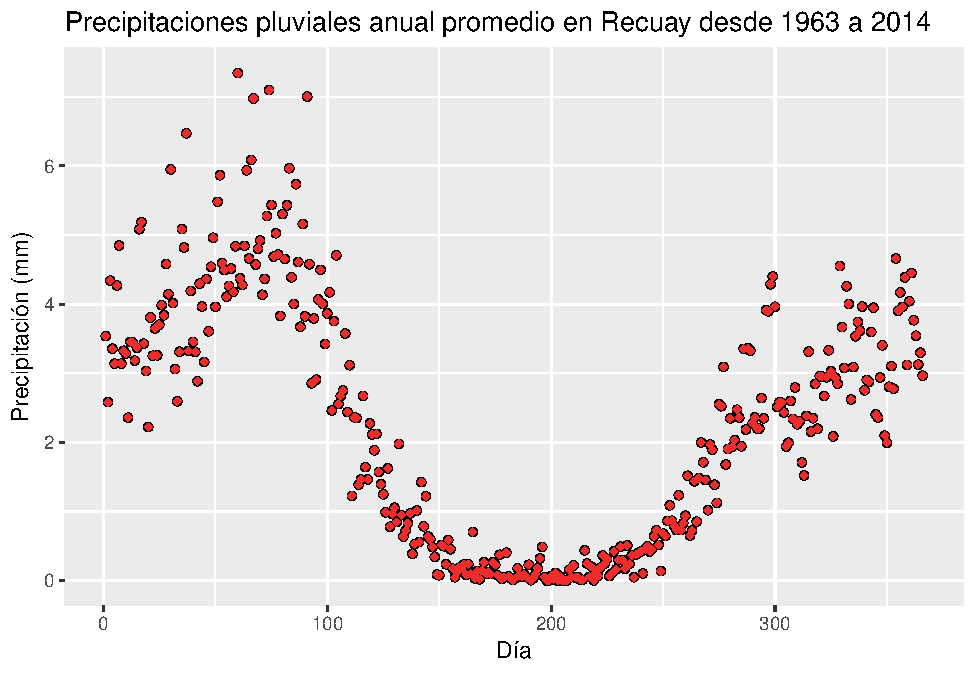
\includegraphics{proyecto_files/figure-latex/unnamed-chunk-6-3.pdf}

\hypertarget{matrices-de-transicion}{%
\subsubsection{Matrices de transición}\label{matrices-de-transicion}}

Para realizar la transición se consideraron dos estados: seco y
lluvioso. Para determinar cuando un día es seco o lluvioso se utilizo
una cuota de 2.5 mm, donde valores superiores iguales a esta cuota
corresponden a un día lluvioso, mientras que valores inferiores al mismo
son considerados secos.

\begin{itemize}
\tightlist
\item
  Día seco: 0
\item
  Día lluvioso: 1
\end{itemize}

\textbf{Nota: Estados considerados}

\begin{itemize}
\tightlist
\item
  Ayer fue seco y hoy fue seco \(P_{00}\): \(1\)
\item
  Ayer fue seco y hoy fue húmedo \(P_{01}\): \(2\)
\item
  Ayer fue húmedo y hoy fue seco \(P_{10}\): \(3\)
\item
  Ayer fue húmedo y hoy fue húmedo \(P_{11}\): \(4\)
\end{itemize}

\textbf{Matriz de transición:}

\[M=\left( \begin{array}{cccc}
 P_{00} & P_{01} \\ 
 P_{10} & P_{11}
\end{array} \right)\]

La siguiente función se hizo para determinar los estados antes
mencionados:

\begin{Shaded}
\begin{Highlighting}[]
\CommentTok{# Determinación de estados}
\NormalTok{conteoCasos<-}\ControlFlowTok{function}\NormalTok{ (data)\{}
\NormalTok{  data}\OperatorTok{$}\NormalTok{V4[data}\OperatorTok{$}\NormalTok{V4}\OperatorTok{<}\FloatTok{2.5}\NormalTok{]<-}\DecValTok{0} 
\NormalTok{  data}\OperatorTok{$}\NormalTok{V4[data}\OperatorTok{$}\NormalTok{V4}\OperatorTok{>=}\FloatTok{2.5}\NormalTok{]<-}\DecValTok{1}
\NormalTok{  tot<-data }\OperatorTok\StringTok{ }\KeywordTok{select}\NormalTok{(}\OperatorTok{-}\NormalTok{V6) }\OperatorTok\StringTok{ }\KeywordTok{filter}\NormalTok{(V4 }\OperatorTok{==}\StringTok{ }\DecValTok{1} \OperatorTok{|}\StringTok{ }\NormalTok{V4 }\OperatorTok{==}\StringTok{ }\DecValTok{0}\NormalTok{) }\CommentTok{##obviamos NAs}
\NormalTok{  tot}\OperatorTok{$}\NormalTok{V5[}\DecValTok{1}\NormalTok{]<-}\DecValTok{0} \CommentTok{#el primer día tiene valor cero}
  \ControlFlowTok{for}\NormalTok{ (i }\ControlFlowTok{in} \DecValTok{2}\OperatorTok{:}\KeywordTok{nrow}\NormalTok{(tot))\{}
    \ControlFlowTok{if}\NormalTok{ (tot}\OperatorTok{$}\NormalTok{V4[i}\DecValTok{-1}\NormalTok{]}\OperatorTok{==}\DecValTok{0} \OperatorTok{&}\StringTok{ }\NormalTok{tot}\OperatorTok{$}\NormalTok{V4[i]}\OperatorTok{==}\DecValTok{0}\NormalTok{)\{ }\CommentTok{#P00}
\NormalTok{      tot}\OperatorTok{$}\NormalTok{V5[i]<-}\DecValTok{1}
\NormalTok{    \} }\ControlFlowTok{else} \ControlFlowTok{if}\NormalTok{(tot}\OperatorTok{$}\NormalTok{V4[i}\DecValTok{-1}\NormalTok{]}\OperatorTok{==}\DecValTok{0} \OperatorTok{&}\StringTok{ }\NormalTok{tot}\OperatorTok{$}\NormalTok{V4[i]}\OperatorTok{==}\DecValTok{1}\NormalTok{)\{ }\CommentTok{#P01}
\NormalTok{      tot}\OperatorTok{$}\NormalTok{V5[i]<-}\DecValTok{2}
\NormalTok{    \} }\ControlFlowTok{else} \ControlFlowTok{if}\NormalTok{ (tot}\OperatorTok{$}\NormalTok{V4[i}\DecValTok{-1}\NormalTok{]}\OperatorTok{==}\DecValTok{1} \OperatorTok{&}\StringTok{ }\NormalTok{tot}\OperatorTok{$}\NormalTok{V4[i]}\OperatorTok{==}\DecValTok{0}\NormalTok{)\{ }\CommentTok{#P10}
\NormalTok{      tot}\OperatorTok{$}\NormalTok{V5[i]<-}\DecValTok{3}
\NormalTok{    \}}\ControlFlowTok{else} \ControlFlowTok{if}\NormalTok{(tot}\OperatorTok{$}\NormalTok{V4[i}\DecValTok{-1}\NormalTok{]}\OperatorTok{==}\DecValTok{1} \OperatorTok{&}\StringTok{ }\NormalTok{tot}\OperatorTok{$}\NormalTok{V4[i]}\OperatorTok{==}\DecValTok{1}\NormalTok{)\{ }\CommentTok{#P11}
\NormalTok{      tot}\OperatorTok{$}\NormalTok{V5[i]<-}\DecValTok{4}
\NormalTok{    \}}
\NormalTok{  \}}
  \KeywordTok{return}\NormalTok{ (tot)}
\NormalTok{\}}
\end{Highlighting}
\end{Shaded}

\begin{Shaded}
\begin{Highlighting}[]
\CommentTok{#Función de conteo y probabilidad de cada estado de la matriz de transición}
\NormalTok{probabilidades<-}\ControlFlowTok{function}\NormalTok{(data)\{}
\NormalTok{  dta <-}\StringTok{ }\KeywordTok{conteoCasos}\NormalTok{(data) }\OperatorTok\StringTok{ }\KeywordTok{filter}\NormalTok{(V5 }\OperatorTok{!=}\DecValTok{0}\NormalTok{) }\CommentTok{#eliminamos primer día}
\NormalTok{    uno <-dta }\OperatorTok\StringTok{ }\KeywordTok{group_by}\NormalTok{(V2) }\OperatorTok\StringTok{ }\KeywordTok{filter}\NormalTok{(V5}\OperatorTok{==}\DecValTok{1}\NormalTok{) }\OperatorTok\StringTok{ }\KeywordTok{summarise}\NormalTok{(}\DataTypeTok{uno=}\KeywordTok{n}\NormalTok{())}
\NormalTok{    dos <-dta }\OperatorTok\StringTok{ }\KeywordTok{group_by}\NormalTok{(V2) }\OperatorTok\StringTok{ }\KeywordTok{filter}\NormalTok{(V5}\OperatorTok{==}\DecValTok{2}\NormalTok{) }\OperatorTok\StringTok{ }\KeywordTok{summarise}\NormalTok{(}\DataTypeTok{dos=}\KeywordTok{n}\NormalTok{())}
\NormalTok{    tres <-dta }\OperatorTok\StringTok{ }\KeywordTok{group_by}\NormalTok{(V2) }\OperatorTok\StringTok{ }\KeywordTok{filter}\NormalTok{(V5}\OperatorTok{==}\DecValTok{3}\NormalTok{) }\OperatorTok\StringTok{ }\KeywordTok{summarise}\NormalTok{(}\DataTypeTok{tres=}\KeywordTok{n}\NormalTok{())}
\NormalTok{    cuatro <-dta }\OperatorTok\StringTok{ }\KeywordTok{group_by}\NormalTok{(V2) }\OperatorTok\StringTok{ }\KeywordTok{filter}\NormalTok{(V5}\OperatorTok{==}\DecValTok{4}\NormalTok{) }\OperatorTok\StringTok{ }\KeywordTok{summarise}\NormalTok{(}\DataTypeTok{cuatro=}\KeywordTok{n}\NormalTok{())}
    
\NormalTok{  resultado <-}\StringTok{ }\KeywordTok{merge}\NormalTok{(}\KeywordTok{merge}\NormalTok{(}\KeywordTok{merge}\NormalTok{(uno, dos, }\StringTok{"V2"}\NormalTok{), tres, }\StringTok{"V2"}\NormalTok{), cuatro, }\StringTok{"V2"}\NormalTok{) }\OperatorTok
\StringTok{    }
\StringTok{  }\KeywordTok{mutate}\NormalTok{(}\DataTypeTok{seco =}\NormalTok{ uno }\OperatorTok{+}\StringTok{ }\NormalTok{dos, }\DataTypeTok{lluvioso =}\NormalTok{ tres }\OperatorTok{+}\StringTok{ }\NormalTok{cuatro) }\OperatorTok\StringTok{ }
\StringTok{    }\KeywordTok{group_by}\NormalTok{(V2) }\OperatorTok\StringTok{ }\KeywordTok{summarise}\NormalTok{(}\DataTypeTok{pUno =}\NormalTok{ uno}\OperatorTok{/}\NormalTok{seco, }\DataTypeTok{pDos =}\NormalTok{ dos}\OperatorTok{/}\NormalTok{seco, }\DataTypeTok{pTres =}\NormalTok{ tres}\OperatorTok{/}\NormalTok{lluvioso,}
    \DataTypeTok{pCuatro =}\NormalTok{ cuatro}\OperatorTok{/}\NormalTok{lluvioso) }\OperatorTok\StringTok{ }\KeywordTok{select}\NormalTok{(}\OperatorTok{-}\NormalTok{V2) }\OperatorTok\KeywordTok{round}\NormalTok{(}\DataTypeTok{digits =} \DecValTok{3}\NormalTok{)}\OperatorTok\StringTok{ }\KeywordTok{as.matrix}\NormalTok{()}
  \KeywordTok{return}\NormalTok{ (resultado)}
\NormalTok{\}}
\end{Highlighting}
\end{Shaded}

\begin{Shaded}
\begin{Highlighting}[]
\CommentTok{# Formateo a listas de las matrices de transición para cada mes}
\NormalTok{propaMatriz <-}\StringTok{ }\ControlFlowTok{function}\NormalTok{(data)\{}
\NormalTok{  prop <-}\StringTok{ }\KeywordTok{probabilidades}\NormalTok{(data)}
\NormalTok{  start <-}\StringTok{ }\KeywordTok{list}\NormalTok{(}\KeywordTok{matrix}\NormalTok{(}\DataTypeTok{nrow =} \DecValTok{2}\NormalTok{, }\DataTypeTok{ncol =} \DecValTok{2}\NormalTok{, }\KeywordTok{c}\NormalTok{(prop[}\DecValTok{1}\NormalTok{,}\DecValTok{1}\NormalTok{],prop[}\DecValTok{1}\NormalTok{,}\DecValTok{2}\NormalTok{],}
\NormalTok{                                             prop[}\DecValTok{1}\NormalTok{,}\DecValTok{3}\NormalTok{], prop[}\DecValTok{1}\NormalTok{,}\DecValTok{4}\NormalTok{]), }\DataTypeTok{byrow =} \OtherTok{TRUE}\NormalTok{))}
  \ControlFlowTok{for}\NormalTok{(i }\ControlFlowTok{in} \DecValTok{2}\OperatorTok{:}\DecValTok{12}\NormalTok{)\{}
\NormalTok{    new <-}\KeywordTok{list}\NormalTok{(}\KeywordTok{matrix}\NormalTok{(}\DataTypeTok{nrow =} \DecValTok{2}\NormalTok{, }\DataTypeTok{ncol =} \DecValTok{2}\NormalTok{, }\KeywordTok{c}\NormalTok{(prop[i,}\DecValTok{1}\NormalTok{],prop[i,}\DecValTok{2}\NormalTok{],}
\NormalTok{                                            prop[i,}\DecValTok{3}\NormalTok{], prop[i,}\DecValTok{4}\NormalTok{]), }\DataTypeTok{byrow =} \OtherTok{TRUE}\NormalTok{))}
\NormalTok{    start <-}\StringTok{ }\KeywordTok{c}\NormalTok{(start, new)}
\NormalTok{  \}}
  \KeywordTok{return}\NormalTok{ (start)}
\NormalTok{\}}
\end{Highlighting}
\end{Shaded}

\begin{Shaded}
\begin{Highlighting}[]
\CommentTok{#Función para estabilizar la matriz en 2^n }
\NormalTok{estabilizar <-}\StringTok{ }\ControlFlowTok{function}\NormalTok{(data, n)\{}
\NormalTok{  matrices <-}\StringTok{ }\KeywordTok{propaMatriz}\NormalTok{(data)}
  \ControlFlowTok{for}\NormalTok{ (j }\ControlFlowTok{in} \DecValTok{1}\OperatorTok{:}\NormalTok{n)\{}
    \ControlFlowTok{for}\NormalTok{ (i }\ControlFlowTok{in} \DecValTok{1}\OperatorTok{:}\DecValTok{12}\NormalTok{)\{}
\NormalTok{      matrices[[i]] <-}\StringTok{ }\NormalTok{matrices[[i]] }\OperatorTok\StringTok{ }\NormalTok{matrices[[i]]}
\NormalTok{    \}}
\NormalTok{  \}}
  \KeywordTok{return}\NormalTok{ (matrices)}
\NormalTok{\}}
\end{Highlighting}
\end{Shaded}

\begin{Shaded}
\begin{Highlighting}[]
\CommentTok{#Limiting probabilities}
\NormalTok{limiting <-}\StringTok{ }\ControlFlowTok{function}\NormalTok{(data, n)\{}
\NormalTok{  matrices <-}\StringTok{ }\KeywordTok{estabilizar}\NormalTok{(data, n)}
\NormalTok{  matrices[[}\DecValTok{1}\NormalTok{]] <-}\StringTok{ }\KeywordTok{matrix}\NormalTok{(}\DataTypeTok{nrow =} \DecValTok{1}\NormalTok{, }\DataTypeTok{ncol=}\DecValTok{2}\NormalTok{, }\KeywordTok{c}\NormalTok{(}\DecValTok{1}\NormalTok{,}\DecValTok{0}\NormalTok{), }\DataTypeTok{byrow =} \OtherTok{TRUE}\NormalTok{) }\OperatorTok\StringTok{ }\NormalTok{matrices[[}\DecValTok{1}\NormalTok{]]}
\NormalTok{  first<-}\KeywordTok{cbind}\NormalTok{(}\KeywordTok{as.data.frame}\NormalTok{(month.abb[}\DecValTok{1}\NormalTok{]), }\KeywordTok{as.data.frame}\NormalTok{(matrices[[}\DecValTok{1}\NormalTok{]]))}
  \KeywordTok{names}\NormalTok{(first)<-}\StringTok{ }\KeywordTok{c}\NormalTok{(}\StringTok{"Mes"}\NormalTok{, }\StringTok{"Seco"}\NormalTok{, }\StringTok{"Húmedo")}
\StringTok{      for (i in 2:12)\{}
\StringTok{      matrices[[i]] <- matrix(nrow = 1, ncol=2, c(1,0), byrow = TRUE) %*% matrices[[i]]}
\StringTok{      second <-cbind(as.data.frame(month.abb[i]), as.data.frame(matrices[[i]]))}
\StringTok{      names(second)<- c("}\NormalTok{Mes}\StringTok{", "}\NormalTok{Seco}\StringTok{", "}\NormalTok{Húmedo")}
\NormalTok{      first<-}\KeywordTok{union}\NormalTok{(first, second)}
\NormalTok{      \}}
  
  \KeywordTok{return}\NormalTok{(first)}
\ErrorTok{\}}
\end{Highlighting}
\end{Shaded}

A continuación se muestran las matrices estabilizadas:

\begin{Shaded}
\begin{Highlighting}[]
\CommentTok{#Matriz estabilizada de Milpo}
\KeywordTok{estabilizar}\NormalTok{(milpo,}\DecValTok{4}\NormalTok{)}
\end{Highlighting}
\end{Shaded}

\begin{verbatim}
## [[1]]
##           [,1]      [,2]
## [1,] 0.4712242 0.5287758
## [2,] 0.4712219 0.5287781
## 
## [[2]]
##           [,1]      [,2]
## [1,] 0.4077725 0.5922275
## [2,] 0.4077632 0.5922368
## 
## [[3]]
##           [,1]      [,2]
## [1,] 0.4107426 0.5892574
## [2,] 0.4107425 0.5892575
## 
## [[4]]
##           [,1]      [,2]
## [1,] 0.5884562 0.4115438
## [2,] 0.5884518 0.4115482
## 
## [[5]]
##           [,1]      [,2]
## [1,] 0.8436268 0.1563732
## [2,] 0.8436268 0.1563732
## 
## [[6]]
##           [,1]       [,2]
## [1,] 0.9377916 0.06220839
## [2,] 0.9377915 0.06220846
## 
## [[7]]
##          [,1]       [,2]
## [1,] 0.952381 0.04761905
## [2,] 0.952381 0.04761905
## 
## [[8]]
##           [,1]       [,2]
## [1,] 0.9261864 0.07381360
## [2,] 0.9261850 0.07381502
## 
## [[9]]
##           [,1]      [,2]
## [1,] 0.7793348 0.2206652
## [2,] 0.7793335 0.2206665
## 
## [[10]]
##           [,1]      [,2]
## [1,] 0.6274517 0.3725483
## [2,] 0.6274498 0.3725502
## 
## [[11]]
##           [,1]      [,2]
## [1,] 0.6202541 0.3797459
## [2,] 0.6202516 0.3797484
## 
## [[12]]
##           [,1]      [,2]
## [1,] 0.5251006 0.4748994
## [2,] 0.5250921 0.4749079
\end{verbatim}

\begin{Shaded}
\begin{Highlighting}[]
\CommentTok{#Matriz estabilizada de Pira}
\KeywordTok{estabilizar}\NormalTok{(pira, }\DecValTok{4}\NormalTok{)}
\end{Highlighting}
\end{Shaded}

\begin{verbatim}
## [[1]]
##           [,1]      [,2]
## [1,] 0.5727672 0.4272328
## [2,] 0.5726737 0.4273263
## 
## [[2]]
##           [,1]      [,2]
## [1,] 0.4499154 0.5500846
## [2,] 0.4498754 0.5501246
## 
## [[3]]
##           [,1]      [,2]
## [1,] 0.3850497 0.6149503
## [2,] 0.3850449 0.6149551
## 
## [[4]]
##           [,1]      [,2]
## [1,] 0.6359062 0.3640938
## [2,] 0.6359057 0.3640943
## 
## [[5]]
##           [,1]       [,2]
## [1,] 0.9006735 0.09932655
## [2,] 0.9006729 0.09932709
## 
## [[6]]
##           [,1]       [,2]
## [1,] 0.9840000 0.01600000
## [2,] 0.9839998 0.01600015
## 
## [[7]]
##           [,1]        [,2]
## [1,] 0.9900990 0.009900987
## [2,] 0.9900987 0.009901324
## 
## [[8]]
##           [,1]       [,2]
## [1,] 0.9799636 0.02003637
## [2,] 0.9799607 0.02003930
## 
## [[9]]
##           [,1]       [,2]
## [1,] 0.9225965 0.07740351
## [2,] 0.9225661 0.07743390
## 
## [[10]]
##           [,1]      [,2]
## [1,] 0.7525834 0.2474166
## [2,] 0.7525589 0.2474411
## 
## [[11]]
##           [,1]      [,2]
## [1,] 0.7136743 0.2863257
## [2,] 0.7136119 0.2863881
## 
## [[12]]
##           [,1]      [,2]
## [1,] 0.6826816 0.3173184
## [2,] 0.6826521 0.3173479
\end{verbatim}

\begin{Shaded}
\begin{Highlighting}[]
\CommentTok{#Matriz estabilizada de Recuay}
\KeywordTok{estabilizar}\NormalTok{(recuay, }\DecValTok{4}\NormalTok{)}
\end{Highlighting}
\end{Shaded}

\begin{verbatim}
## [[1]]
##           [,1]      [,2]
## [1,] 0.5960452 0.4039548
## [2,] 0.5960452 0.4039548
## 
## [[2]]
##          [,1]     [,2]
## [1,] 0.526087 0.473913
## [2,] 0.526087 0.473913
## 
## [[3]]
##           [,1]      [,2]
## [1,] 0.4766484 0.5233516
## [2,] 0.4766484 0.5233516
## 
## [[4]]
##          [,1]     [,2]
## [1,] 0.654047 0.345953
## [2,] 0.654047 0.345953
## 
## [[5]]
##           [,1]      [,2]
## [1,] 0.8865248 0.1134752
## [2,] 0.8865248 0.1134752
## 
## [[6]]
##           [,1]       [,2]
## [1,] 0.9756637 0.02433628
## [2,] 0.9756637 0.02433628
## 
## [[7]]
##           [,1]       [,2]
## [1,] 0.9896074 0.01039261
## [2,] 0.9896074 0.01039261
## 
## [[8]]
##           [,1]       [,2]
## [1,] 0.9625963 0.03740374
## [2,] 0.9625963 0.03740374
## 
## [[9]]
##           [,1]      [,2]
## [1,] 0.8657718 0.1342282
## [2,] 0.8657718 0.1342282
## 
## [[10]]
##           [,1]      [,2]
## [1,] 0.6788219 0.3211781
## [2,] 0.6788219 0.3211781
## 
## [[11]]
##           [,1]      [,2]
## [1,] 0.6953243 0.3046757
## [2,] 0.6953243 0.3046757
## 
## [[12]]
##           [,1]      [,2]
## [1,] 0.6316615 0.3683385
## [2,] 0.6316614 0.3683386
\end{verbatim}

Finalmente, los vectores estabilizados y limitados para cada estación
metereológica se detalla a continuación:

\begin{Shaded}
\begin{Highlighting}[]
\CommentTok{#Vector estabilizada de Milpo}
\KeywordTok{limiting}\NormalTok{(milpo,}\DecValTok{4}\NormalTok{)}
\end{Highlighting}
\end{Shaded}

\begin{Shaded}
\begin{Highlighting}[]
\CommentTok{#Vector estabilizada de Pira}
\KeywordTok{limiting}\NormalTok{(pira,}\DecValTok{4}\NormalTok{)}
\end{Highlighting}
\end{Shaded}

\begin{Shaded}
\begin{Highlighting}[]
\CommentTok{#Vector estabilizada de Recuay}
\KeywordTok{limiting}\NormalTok{(recuay,}\DecValTok{4}\NormalTok{)}
\end{Highlighting}
\end{Shaded}


\end{document}
